\chapter{Polynomiumsinterpolation} \label{interpolation}

Den endelige element løsning er som bekendt en linearkombination af en
række polynomier fra et vist løsningsrum. Når man skal udføre
fejlestimering, er det derfor vigtigt at vide, hvor godt man kan
approksimere funktioner med polynomier fra det valgte løsningsrum. Ofte er
fejlestimatorer og dermed polynomiumsinterpolation drivkraften bag
netinddelings algoritmer. I næste kapitel skal vi studere en
netinddelings algoritme, der gør brug af en bestemt fejlligning, som
vi derfor skal verificere i dette kapitel. Det skal bemærkes, at vi
ikke er interesseret i den bedste polynomiums interpolant, men derimod
mere interesseret i at opnå en fejlligning på en bestemt form.
Interpolationsteori, hvor man forsøger at få den bedst mulige
approksimation, er fx behandlet i \cite{chen1,chen2}. Generel
interpolationsteori for vilkårlige Sobolev rum kan fx findes i
\cite{ciarlet78}.

\section{A priori fejlligningen}
Som nævnt ovenfor er vi interesseret i en ganske bestemt fejlligning.
Mere præcist ønsker vi at udtrykke interpolations fejlen på formen
\begin{equation}
  \norm{e}^q = \sum_{i=1}^k \phi_i h_x^{\gamma_{1,i}}
  h_y^{\gamma_{2,i}} + \hot
\end{equation}
Vi skal studere tilfældet, hvor det to dimensionale fysiske domæne er
blevet afbildet bijektivt på et passende antal kvadrater, og hvor de
endelige elementer (i kvadraterne) består af akseparallelle rektangler
med sidelængde $h_x$ og $h_y$. Funktionerne $\phi_i$ må gerne afhænge
af den funktion, vi ønsker at interpolere, men ikke af de endelige
elementers geometri. Konstanterne $q$, $\gamma_{j,i}$ og $k$ er
passende norm afhængige konstanter, og $\hot$ betegner højere ordens
led.

Lad $\re =[a,a+h_x]\times [b,b+h_y]$ være et rektangel i $\R^2$. Vi
skal da betragte approksimationer til funktioner $u:\re\subset\R^2
\rightarrow \R^2$ med polynomier fra produktrummet $Q_{pq}$ givet ved
\begin{equation}
  Q_{pq} = \spann \{\varphi_{ij} : (x,y)\rightarrow x^i y^j \in\R \ |\
  0\leq i\leq p, \ 0\leq j\leq q \}.
\end{equation}
Vi skal antage, at $u$ er tilstrækkelig differentiabel til, at vi kan
foretage en Taylor udvikling af $(p+2)\times(q+2)$'te orden med restled i
ethvert punkt $(x_0,y_0)\in\re$, dvs.
\begin{equation}
  u(x,y) =  \sum_{i=0}^{p+2} \sum_{j=0}^{q+2} \phi_{ij}(x,y) +
  R_{p+2,q+2}(x,y),
\end{equation}
hvor
\begin{gather}
  \phi_{ij}(x,y) =
  \frac{1}{i!j!}\frac{\p^{i+j}u(x_0,y_0)}{\p x^i \p y^j}
  (x-x_0)^i(y-y_0)^j, \\
  R_{p+2,q+2}(x,y) =
  \sum_{k=0}^{q+3} \OO_{h_x,h_y\rightarrow 0} (h_x^{p+3}h_y^k) +
  \sum_{k=0}^{p+3} \OO_{h_x,h_y\rightarrow 0} (h_x^kh_y^{p+3}). \label{restled}
\end{gather}
Notationen i \eqref{restled} indikerer, at vi hovedsageligt er interesseret i
det asymptotiske tilfælde, hvor $h_x \rightarrow 0$ og $h_y
\rightarrow 0$.

\section{Lokal Taylor po\-ly\-no\-mi\-ums in\-ter\-po\-la\-ti\-on i et rek\-tan\-gel i $\R^2$}
Med notationen fra forrige afsnit skal vi definere Taylor polynomiums
interpolanten af $u$ af grad $p$ i $x$ og af grad $q$ i $y$ som
\begin{equation}
  T_{pq}\{u\}(x,y) = \sum_{i=0}^{p} \sum_{j=0}^{q} \phi_{ij}(x,y).
\end{equation}
Fejlen, vi begår ved at approksimere $u$ med $T_{pq}\{u\}$, defineres som
\begin{equation}
  e_{pq}^T = u - T_{pq}\{u\}.
\end{equation}
I figur~\ref{grafisk} er en grafisk illustration af $u$ opsplittet i
$\Tayu$ og $\Taye$.
\begin{figure}[htb]
\begin{displaymath}
% \setlength{\extrarowheight}{2pt}
\begin{array}{|ccc|cc|c|}
 \hline \phi_{00} & \cdots & \phi_{p0} & \phi_{p+1,0}
          & \phi_{p+2,0} & \OO (h_x^{p+3}h_y^0) \\
        \vdots & & \vdots & \vdots & \vdots & \vdots \\
        \phi_{0q} & \cdots & \phi_{pq} & \phi_{p+1,q}
          & \phi_{p+2,q} & \OO (h_x^{p+3}h_y^q) \\
 \hline \phi_{0,q+1} & \cdots & \phi_{p,q+1} & \phi_{p+1,q+1}
          & \phi_{p+2,q+1} & \OO (h_x^{p+3}h_y^{q+1}) \\
        \phi_{0,q+2} & \cdots & \phi_{p,q+2} & \phi_{p+1,q+2}
          & \phi_{p+2,q+2} & \OO (h_x^{p+3}h_y^{q+2}) \\
 \hline \OO (h_x^0 h_y^{q+3}) & \cdots & \OO (h_x^p h_y^{q+3})
          & \OO (h_x^{p+1} h_y^{q+3}) & \OO (h_x^{p+2} h_y^{q+3})
            & \OO (h_x^{p+3} h_y^{q+3}) \\
 \hline
\end{array}
\end{displaymath}
\begin{displaymath}
\begin{array}{|cccccc|}
 \hline
 \multicolumn{3}{|c|}{} & \multicolumn{3}{|c|}{}  \\
 \multicolumn{3}{|c|}{T_{pq}\{u\}} & \multicolumn{3}{|c|}{}  \\
 \multicolumn{3}{|c|}{} & \multicolumn{3}{|c|}{}  \\ \cline{1-3}
 & & & \multicolumn{2}{c}{e_{pq}^T}   & \\
 & & & & & \\
        \phantom{\O (h_x^0 h_y^{q+3})} &
        \phantom{\cdots} &
        \phantom{\O (h_x^p h_y^{q+3})} &
        \phantom{\O (h_x^{p+1} h_y^{q+3})} &
        \phantom{\O (h_x^{p+2} h_y^{q+3})} &
        \phantom{\O (h_x^{p+3} h_y^{q+3})} \\
 \hline
\end{array}
\end{displaymath}
\caption{Grafisk illustration af $u$ opsplittet i $\Tayu$ og $\Taye$\label{grafisk}}
\end{figure}
For at undgå udartede rektangler skal vi antage, at der er en
sammenhæng mellem sidebredden og -længden. Mere formelt skal vi
forudsætte, at der findes en global konstant $H$, så der for alle
rektangler i netinddelingen findes et $s\in[1/H,H]$, så
\begin{equation}
  h_x=h, \quad h_y=sh.
\end{equation}
Vi skal senere udnytte, at dette krav medfører $h_x \approx h_y$ for
$h_x\rightarrow 0$ og $h_y\rightarrow 0$.

Ved nu at bemærke, at $\phi_{ij} = \OO_{h_x,h_y\rightarrow 0}(h_x^ih_y^j)
= \OO_{h\rightarrow 0}(h^{i+j})$ for vilkårlige ikke-negative tal $i$
og $j$ fås følgende relation for $\Taye$
\begin{equation} \label{fejl1}
e_{pq}^T =
  \begin{cases}
    \{ \un{\phi_{p+1,0}} + \un{\phi_{0,q+1}} \} + \hot
      & \text{for $p=q$,} \\
    \{ \un{\phi_{p+1,0}} \} + \{ \phi_{p+2,0} + \phi_{p+1,1}
      + \un{\phi_{0,q+1}} \} + \hot & \text{for $p=q-1$,} \\
    \{ \un{\phi_{0,q+1}} \} + \{ \phi_{0,q+2} + \phi_{1,q+1}
      + \un{\phi_{p+1,0}} \} + \hot & \text{for $p=q+1$,} \\
    \{ \un{\phi_{p+1,0}} \} + \{ \phi_{p+2,0} +
      \un{\phi_{p+1,1}} \} + \hot & \text{for $p<q-1$,} \\
    \{ \un{\phi_{0,q+1}} \} + \{ \phi_{0,q+2} +
      \un{\phi_{1,q+1}} \} + \hot & \text{for $p>q+1$.}
  \end{cases}
\end{equation}
Vi har her brugt betegnelsen $\hot$ om højere ordens led i $h$ (eller
i $h_x$ og $h_y$). For at forklare betydningen af de understregede led
i \eqref{fejl1} skal vi betragte følgende eksempel:

\begin{example}
Betragt funktionen $u(x,y)=\cos Kx \cos y$ for et passende $K\gg 1$,
og lad $\re=[0,h_x]\times [0,h_y]$, $(x_0,y_0)=(h_x/2,h_y/2)$ samt
$p=q+1=1$. Vi har valgt $p>q$, da $u$ varierer hurtigere i
$x$-retningen end i $y$-retningen.  Fra \eqref{fejl1} fås
\begin{equation}
  e_{pq}^T = \{ \un{\phi_{0,q+1}} \} + \{ \phi_{0,q+2} +
  \phi_{1,q+1} + \un{\phi_{p+1,0}} \} + \hot,
\end{equation}
hvor vi i dette tilfælde finder
\begin{gather}
  \phi_{0,q+1} = -\cos (Kh_x/2) \sin (h_y/2) (y-h_y/2), \\
  \phi_{0,q+2} = -\frac{1}{2} \cos (Kh_x/2) \cos (h_y/2) (y-h_y/2)^2, \\
  \phi_{1,q+1} = K \sin (Kh_x/2) \sin (h_y/2) (x-h_x/2)(y-h_y/2), \\
  \phi_{p+1,0} = -\frac{K^2}{2}\cos (Kh_x/2) \cos (h_y/2) (x-h_x/2)^2,
\end{gather}
Udnyttes nu, at $|\sin t\, |\leq 1$, $|\cos t\, |\leq 1$,
$|x-h_x/2|\leq h_x/2$ og $|y-h_y/2|\leq h_y/2$, fås
\begin{equation} \label{est-fejl1}
  |e_{pq}^T| \leq \frac{1}{2}h_y + \frac{1}{2\cdot 4}h_y^2 +
  \frac{K}{2\cdot 2}h_xh_y + \frac{K^2}{2\cdot 4}h_x^2 + \hot
\end{equation}
Som nævnt ovenfor er vores mål at have $h_x \approx h_y$. Ved
at indsætte $h_x =h$ og $h_y =sh$ i \eqref{est-fejl1} ses, at
\begin{equation}
  |e_{pq}^T| \leq \frac{1}{2}h + \frac{s^2}{2\cdot 4}h^2 +
  \frac{Ks}{2\cdot 2}h^2 + \frac{K^2}{2\cdot 4}h^2 + \hot
\end{equation}
I denne ligning er det klart, at leddet af størrelsesorden $h$
dominerer for $h\rightarrow 0$, og idet $K\gg 1$ vil det sidste led
dominere de andre $h^2$ led. Eller sagt med andre ord: De dominerede
led i $\Taye$ er $\phi_{0,q+1}$ og $\phi_{p+1,0}$, dvs. de
understregede led.
\begin{figure}
% \psdraft
% \MaplePlotHeight = 6cm
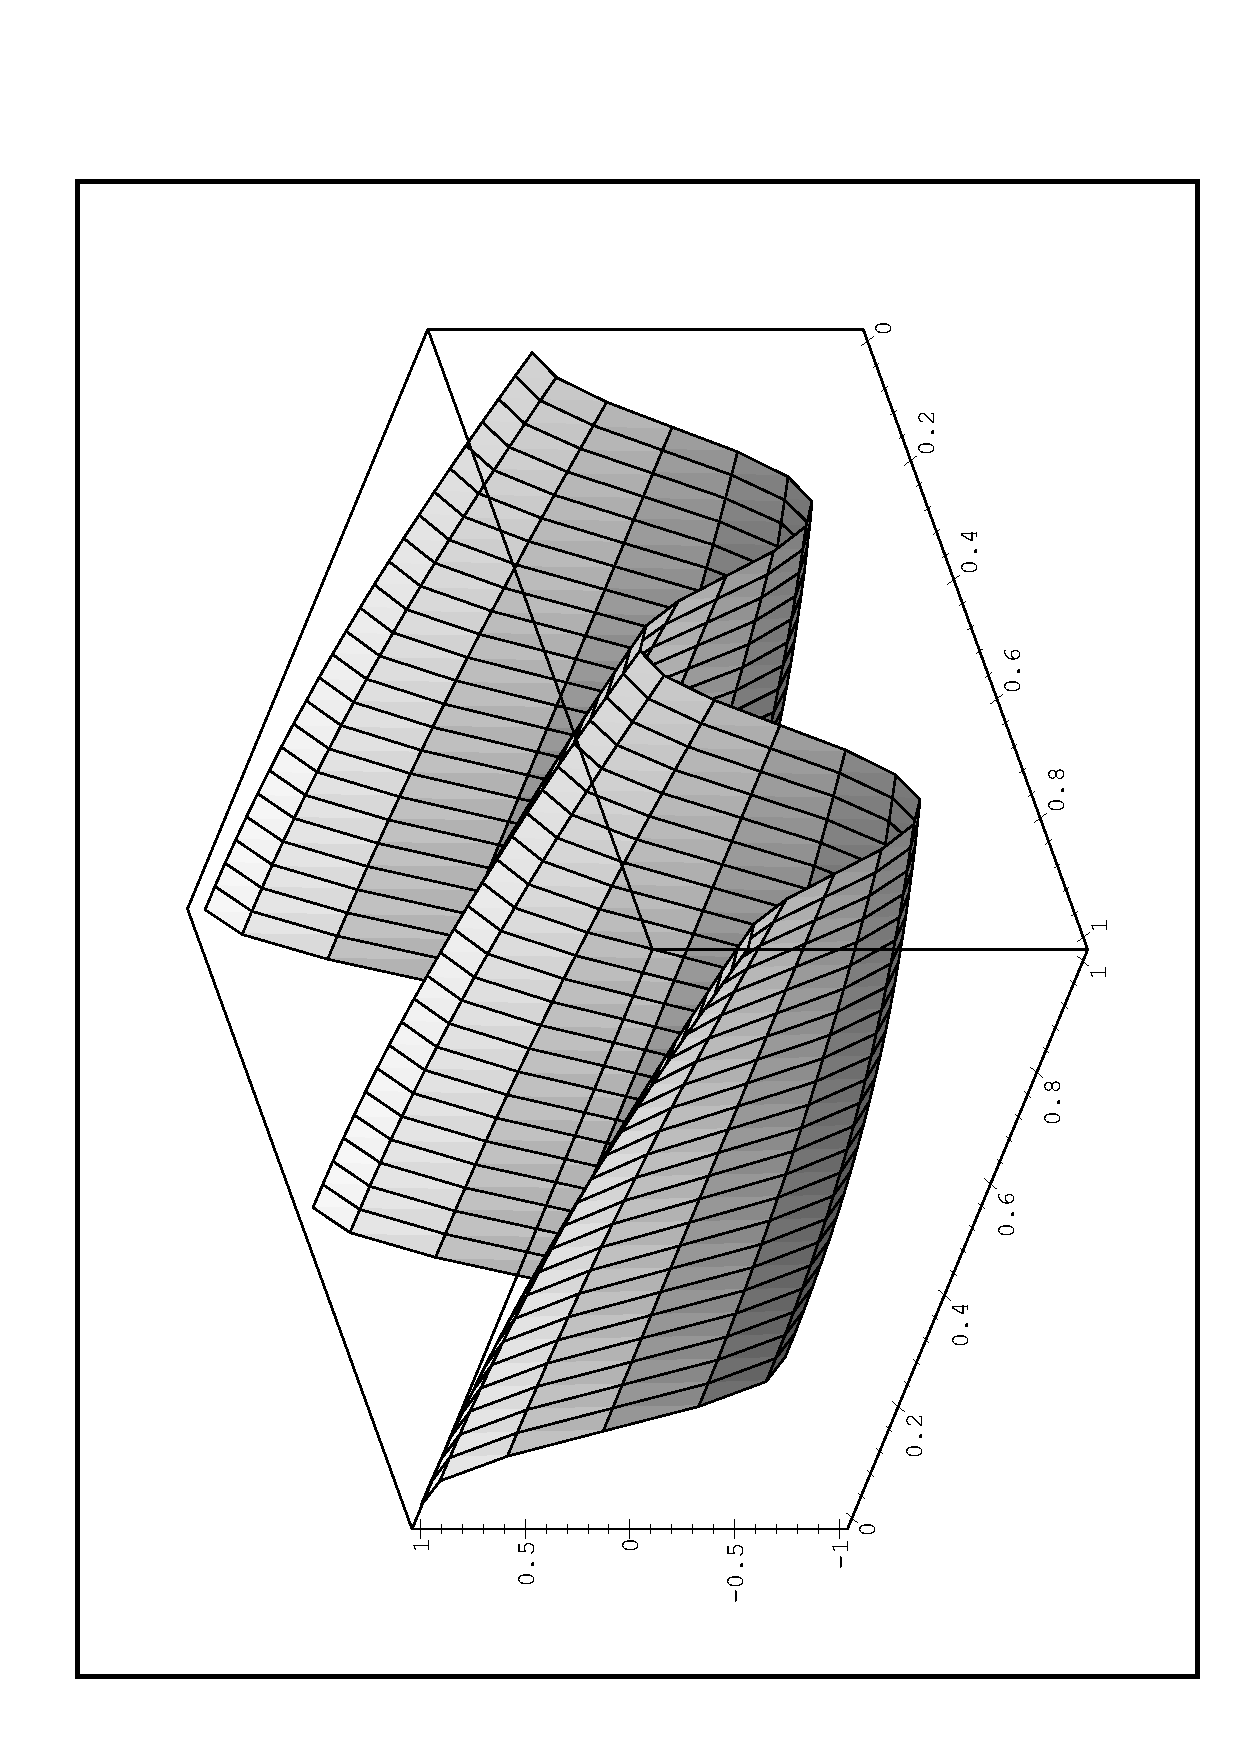
\includegraphics{cos}
\caption{Illustration af $u$ i tilfældet $K = 4\pi$ og
$\re=[0,1]\times [0,1]$.}
\end{figure}
\end{example}
For et eksempel i tilfældet $p=q-1=1$ henvises til \cite{hugger-pol}. Disse
eksempler giver os følgende formodning.
\begin{conjecture} \label{konjektur}
Vælges $p$ og $q$ forskelligt på grund af en hurtigere variation i $u$
i enten $x$-retningen eller i $y$-retningen, og har vi som overordnet mål
at opnå $h_x = h \approx h_y = sh$, da vil de dominerende led i
$\Taye$ for $h\rightarrow 0$, være de understregede led i ligningen \eqref{fejl1}.
\end{conjecture}

Ved kun medtage de dominerende led fra ligning \eqref{fejl1} fås følgende
udtryk for $\Taye$.
\begin{equation} \label{fejl2}
e_{pq}^T =
  \begin{cases}
    \phi_1 h_x^{p+1} + \phi_2 h_y^{q+1} + \hot &
      \text{for $p=q$,} \\
    \phi_1 h_x^{p+1} + \phi_2 h_y^{q+1} + \pst &
      \text{for $p=q-1$,} \\
    \phi_1 h_y^{q+1} + \phi_2 h_x^{p+1} + \pst &
      \text{for $p=q+1$,} \\
    \phi_1 h_x^{p+1} + \phi_2 h_x^{p+1} h_y + \pst &
      \text{for $p<q-1$,} \\
    \phi_1 h_y^{q+1} + \phi_2 h_x h_y^{q+1} + \pst &
      \text{for $p>q+1$.} \\
  \end{cases}
\end{equation}
Funktionerne $\phi_1$ og $\phi_2$ afhænger hverken
af $h_x$ eller af $h_y$, men er ikke nødvendigvis identiske i de
enkelte tilfælde. I overensstemmelse med konjektur~\ref{konjektur} betegner
$\pst$ formodet mindre led.

For at opskrive ${\mathcal W}^{m,r}$ Sobolev normen af fejlen
genkalder vi os først definitionen af denne
\begin{equation} \label{sobolevnorm}
  \snorm{v} = \sum_{\substack{ i,j\geq 0 \\ i+j \leq m}} \int_\re
  \Bigl| \frac{\p^{i+j} v(x,y)}{\p x^i \p y^j} \Bigr|^r\, dx\, dy.
\end{equation}
Som sædvanlig er $v$ en passende funktion, $m$ et ikke negativt tal,
og $r$ et positivt tal. Ved at anvende denne definition på de enkelte
tilfælde i \eqref{fejl2} fås for $m=0$
\begin{equation} \label{fejl3}
  \smnorm{e_{pq}^T}{0} =
  \left\{
  \begin{array}{ll}
  (\phi_1 h_x^{p+1} + \phi_2 h_y^{q+1})^r h_x h_y + \hot &
    \mbox{for $p=q$,} \\
  (\phi_1 h_x^{p+1} + \phi_2 h_y^{q+1})^rh_xh_y + \pst = & \\
  \phi_1 h_x^{(p+1)r+1} h_y + \phi_2 h_x^{(p+1)(r-1)+1} h_y^{q+2} +\pst &
    \mbox{for $p=q-1$,} \\
  (\phi_1 h_y^{q+1} + \phi_2 h_x^{p+1})^r h_x h_y +\pst = & \\
  \phi_1 h_x h_y^{(q+1)r+1} + \phi_2 h_x^{p+2} h_y^{(q+1)(r-1)+1} +\pst &
    \mbox{for $p=q+1$,} \\
  (\phi_1 h_x^{p+1} + \phi_2 h_x^{p+1}h_y)^r h_x h_y +\pst = & \\
  \phi_1 h_x^{(p+1)r+1} h_y + \phi_2 h_x^{(p+1)r+1} h_y^{2}
    +\pst & \mbox{for $p<q-1$,} \\
  (\phi_1 h_y^{q+1} + \phi_2 h_x h_y^{q+1})^r h_x h_y +\pst = & \\
  \phi_1 h_x h_y^{(q+1)r+1} + \phi_2 h_x^{2} h_y^{(q+1)r+1}
    +\pst & \mbox{for $p>q+1$.}
  \end{array}
  \right.
\end{equation}

For at undgå for tung notation har vi her skrevet $\phi_1$ hhv.
$\phi_2$ istedet $\phi_1^r$ hhv. $\phi_2^r$. Når $m\geq 1$ er det ikke
nok kun at betragte de understregede led i \eqref{fejl1}. Lad os som
eksempel betragte tilfældet $m=1$ og $p=q+1$. Her er

\begin{align}
 \snorm{e_{pq}^T} &= ( \phi_1 h_y^{q+1} + \phi_2 h_x^{p} )^r h_x h_y \\
 &\phantom{= (} + ( \phi_3 h_y^q + \phi_4 h_y^{q+1} +
   \phi_5 h_x h_y^q )^r h_x h_y \notag \\
 &\phantom{= (} + ( \phi_6 h_y^{q+1} + \phi_7 h_y^{q+2} +
   \phi_8 h_x h_y^{q+1} + \phi_9 h_x^{p+1} )^r h_x h_y + \hot \notag \\
 &= \phi_1 h_x h_y^{qr+1} + \phi_2 h_x^2 h_y^{qr+1} + \pst \notag
\end{align}

Her har vi igen ``misbrugt'' notationen forstået på den måde, at
$\phi_1$ hhv. $\phi_2$ i det endelige resultat, ikke er det samme
$\phi_1$ og $\phi_2$ som i den første ligning. De øvrige tilfælde fås
på lignende vis.

\begin{equation} \label{fejl4}
\smnorm{e_{pq}^T}{1} =
\begin{cases}
  \phi_1 h_x^{pr+1} h_y + \phi_2 h_x h_y^{qr+1} + \hot &
    \text{for $p=q$} \\
  \phi_1 h_x^{pr+1} h_y + \phi_2 h_x^{pr+1} h_y^2 + \pst &
    \text{for $p=q-1$} \\
  \phi_1 h_x h_y^{qr+1} + \phi_2 h_x^2 h_y^{qr+1} + \pst &
    \text{for $p=q+1$} \\
  \phi_1 h_x^{pr+1} h_y + \phi_2 h_x^{pr+1} h_y^2 + \pst &
    \text{for $p<q-1$} \\
  \phi_1 h_x h_y^{qr+1} + \phi_2 h_x^2 h_y^{qr+1} + \pst &
    \text{for $p>q+1$} \\
\end{cases}
\end{equation}

For $2\leq m \leq 1 + \min \{ p,q \}$ kan man (igen på tilsvarende
måde) få

\begin{equation} \label{fejl5}
\snorm{e_{pq}^T} =
\begin{cases}
  \phi_1 h_x^{(p+1-m)r+1} h_y + \\
  \phantom{\phi_1 h_x} \phi_2 h_x h_y^{(q+1-m)r+1} + \hot &
    \text{for $p=q$} \\
  h_x^{(p+1-m)r+1}(\phi_1 h_y +\phi_2 h_y^2) + \pst & \text{for $p=q-1$} \\
  h_y^{(q+1-m)r+1}(\phi_1 h_x +\phi_2 h_x^2) + \pst & \text{for $p=q+1$} \\
  h_x^{(p+1-m)r+1}(\phi_1 h_y +\phi_2 h_y^2) + \pst & \text{for $p<q-1$} \\
  h_y^{(q+1-m)r+1}(\phi_1 h_x +\phi_2 h_x^2) + \pst & \text{for $p>q-1$} \\
\end{cases}
\end{equation}

Sammenfattes ovenstående resultater fås følgende sætning.

\begin{theorem} \label{errortheorem}
Lad $p$ og $q$ være positive tal, og antag at $u:\R^2 \rightarrow
\R^2$ er glat nok til at have en Taylor udvikling af orden
$(p+2)\times (q+2)$ med restled i ethvert punkt i et rektangel
$\re\subset\R^2$ med sidelængder $h_x$ og $h_y$. Vi har da følgende
asymptotiske fejlligning for Taylor interpolations polynomier i
$Q_{pq}(\re)$ når $h_x \rightarrow 0$ og $h_y \rightarrow 0$:

Der findes funktioner $\phi_1$ og $\phi_2$ og tal $s_1$, $s_2$, $t_1$
og $t_2$ uafhængige af $h_x$ og $h_y$ men afhængige af $u$, $p$ og $q$
så
\begin{equation} \label{thm-1}
  e_{pq}^T = \phi_1 h_x^{s_1} h_y^{s_2} +
  \phi_2 h_x^{t_1}h_y^{t_2} + \pst ,
\end{equation}
og
\begin{equation} \label{thm-2}
  \snorm{e_{pq}^T} = \phi_1 h_x^{s_1} h_y^{s_2} +
  \phi_2 h_x^{t_1}h_y^{t_2} + \pst .
\end{equation}
Her er $m$ og $r$ tal, som opfylder $0\leq m\leq 1+\min \{ p,q \}$.
Funktionerne $\phi_1$ og $\phi_2$ er ikke nødvendigvis identiske i
\eqref{thm-1} og \eqref{thm-2}, hvilket også gælder for $s_1$, $s_2$, $t_1$
og $t_2$. Værdierne af $s_1$, $s_2$, $t_1$ og $t_2$ er givet fra
ligningerne \eqref{fejl2}, \eqref{fejl3}, \eqref{fejl4} og \eqref{fejl5}.
Er $p=q$ erstattes $\pst$ med $\hot$.
\end{theorem}

Sætning~\ref{errortheorem} giver ikke mange oplysninger om
funktionerne $\phi_1$ og $\phi_2$.
Vi kan få mere præcise oplysninger om disse fra ligning~\eqref{fejl1}. Det er
klart, at vi kan skrive $\Taye$ på formen
\begin{equation} \label{kombination}
  e_{pq}^T = \sum_{k=1}^6 \alpha_k \phi_{p_k,q_k} + \hot\ ,
\end{equation}
hvor konstanterne $\alpha_k, \ k=1,\ldots,6$ enten har værdien $0$ eller
$1$ afhængig af, om den tilhørende funktion $\phi_{p_k,q_k}$ indgår i
ligning~\eqref{fejl1}. Værdierne for $p_k$, $q_k$ og $\alpha_k$ ses i
tabel~\ref{alphavalues}.
\begin{table}[htb]
\begin{displaymath}
\begin{array}{|c|c|cccccc|}
  \hline & & k=1 & k=2 & k=3 & k=4 & k=5 & k=6 \\
  \hline & p_k & p+1 & p+1 & p+2 & 0 & 1 & 0 \\
         & q_k & 0 & 1 & 0 & q+1 & q+1 & q+2 \\
  \hline p=q   & \alpha_k & 1 & 0 & 0 & 1 & 0 & 0 \\
         p=q-1 & \alpha_k & 1 & 1 & 1 & 1 & 0 & 0 \\
         p=q+1 & \alpha_k & 1 & 0 & 0 & 1 & 1 & 1 \\
         p<q-1 & \alpha_k & 1 & 1 & 1 & 0 & 0 & 0 \\
         p>q+1 & \alpha_k & 0 & 0 & 0 & 1 & 1 & 1 \\
  \hline
\end{array}
\end{displaymath}
\caption{Værdierne for $p_k$, $q_k$ og $\alpha_k$ i formlen for $\Taye$\label{alphavalues}}
\end{table}
Ved at anvende \eqref{sobolevnorm}, \eqref{kombination}, multinomial
formlen samt følgende relation mellem normen og seminormen i ${\mathcal W}^{m,r}$
\begin{equation}
  \snorm{e_{pq}^T} =  \ssnorm{e_{pq}^T} + \hot
\end{equation}
hvor
\begin{equation}
  \ssnorm{v} = \sum_{\substack{ i,j\geq 0 \\ i+j = m}} \int_\re
  \Bigl| \frac{\p^{i+j} v(x,y)}{\p x^i \p y^j} \Bigr|^r\, dx\, dy
\end{equation}
ses, at
\begin{equation} \label{normfejl1}
\begin{split}
  \snorm{e_{pq}^T} &= \Bigl\| \sum_{k=1}^6 \alpha_k
  \phi_{p_k,q_k} \Bigr\| + \hot \\
  &= \sum_{\substack{ i,j\geq 0 \\ i+j=m }} \int_\re \Bigl|
  \frac{\p^{i+j}\sum_{k=1}^6 \alpha_k \phi_{p_k,q_k}(x,y)}
  {\p x^i \p y^j} \Bigr|^r\, dx\, dy + \hot \\
  &= \sum_{\substack{ i,j\geq 0 \\ i+j=m }}
  \int_\re \sum_{\substack{ r_1,\ldots ,r_6 \geq 0 \\ r_1+\cdots +r_6=r}} 
  r! \prod_{k=1}^{6} \frac{1}{r_k!}
  \Bigl| \alpha_k \frac{\p^{i+j} \phi_{p_k,q_k}(x,y)}
  {\p x^i \p y^j} \Bigr|^{r_k}\, dx\, dy + \hot \\
\end{split}
\end{equation}
Defineres $F$ som
\begin{equation} \label{F}
\begin{split}
  F(x,y) &= r! \prod_{k=1}^{6} \frac{1}{r_k!}
  \Bigl| \alpha_k \frac{\p^{i+j} \phi_{p_k,q_k}(x,y)}
  {\p x^i \p y^j} \Bigr|^{r_k} \\
  &=  r! \prod_{k=1}^{6} \frac{1}{r_k!}
  \Bigl| \frac{\alpha_k}{p_k!q_k!}
  \frac{\p^{p_k+q_k} u(x_0,y_0)}{\p x^{p_k} \p y^{q_k}}
  \frac{\p^i(x-x_0)^{p_k}}{\p x^i}
  \frac{\p^j(y-y_0)^{q_k}}{\p y^j} \Bigr|^{r_k}, \\
\end{split}
\end{equation}
kan vi skrive \eqref{normfejl1} som
\begin{equation} \label{normfejl2}
  \snorm{e_{pq}^T} = \sum_{\substack{ i,j\geq 0 \\ i+j=m }}
  \sum_{\substack{ r_1,\ldots ,r_6 \geq 0\\ r_1+\cdots +r_6=r}}
  \int_\re F(x,y)\, dx\, dy + \hot .
\end{equation}
Integralet i ligning~\eqref{normfejl2} kan udregnes ved hjælp af
\eqref{F} og giver
\begin{multline} \label{kompl}
  \snorm{e_{pq}^T} \\
\begin{split}
  &= \sum_{\substack{ i,j\geq 0 \\ i+j=m }}
  \sum_{\substack{ r_1,\ldots ,r_6 \geq 0 \\ r_1+\cdots +r_6=r}} \\
  &\qquad  \int_\re r! \prod_{k=1}^6 \frac{1}{r_k!} \Bigl|
  \frac{\alpha_k}{p_k!q_k!} \frac{\p^{p_k+q_k}u(x_0,y_0)}{\p x^{p_k}\p y^{q_k}}
  \frac{\p^i u(x-x_0)^{p_k}}{\p x^i} \frac{\p^j u(y-y_0)^{q_k}}{\p y^j}
  \Bigr|^{r_k}\, dx\, dy + \hot \\
  &= \sum_{\substack{ i,j\geq 0 \\ i+j=m }}
  \sum_{\substack{ r_1,\ldots ,r_6 \geq 0 \\ r_1+\cdots +r_6=r}}
  r! \prod_{k=1}^6 \frac{1}{r_k!} \Bigl|
  \frac{\alpha_k}{p_k!q_k!} \frac{\p^{p_k+q_k}u(x_0,y_0)}{\p x^{p_k}\p y^{q_k}}
  \Bigr|^{r_k} \\
  &\qquad \cdot \int_\re \prod_{k=1}^6 \Bigl|
  \frac{\p^i u(x-x_0)^{p_k}}{\p x^i} \frac{\p^j u(y-y_0)^{q_k}}{\p y^j}
  \Bigr|^{r_k}\, dx\, dy + \hot \\
  &= \sum_{\substack{ i,j\geq 0 \\ i+j=m }}
  \sum_{\substack{ r_1,\ldots ,r_6 \geq 0 \\ r_1+\cdots +r_6=r}}
  r! \prod_{k=1}^6 \frac{1}{r_k!} \Bigl|
  \frac{\alpha_k}{p_k!q_k!} \frac{\p^{p_k+q_k}u(x_0,y_0)}{\p x^{p_k}\p y^{q_k}}
  \Bigr|^{r_k} \\
  &\qquad \cdot \int_{a}^{a+h_x} \prod_{k=1}^6 \Bigl|
  \frac{\p^i u(x-x_0)^{p_k}}{\p x^i} \Bigr|^{r_k}\, dx
  \int_{b}^{b+h_y} \prod_{k=1}^6 \Bigl|
  \frac{\p^j u(y-y_0)^{q_k}}{\p y^j} \Bigr|^{r_k}\, dy + \hot \\
\end{split}
\end{multline}
I det sidste led regner vi på det ene integrale og finder (for
$1\leq i\leq p_k$, $1\leq j\leq q_k$ og $r_k>0$)
\begin{multline}
  \int_{a}^{a+h_x} \prod_{k=1}^6 \Bigl|
  \frac{\p^i (x-x_0)^{p_k}}{\p x^i} \Bigr|^{r_k}\, dx \\
\begin{split}
  &= \int_{a}^{a+h_x} \prod_{k=1}^6 \Bigl| \, \prod_{s=0}^{i-1}
  (p_k-s) (x-x_0)^{p_k-i}\Bigl|^{r_k}\, dx \\
  &= \prod_{k=1}^6 \prod_{s=0}^{i-1} (p_k-s)^{r_k}
  \int_{a}^{a+h_x} \prod_{k=1}^6 |x-x_0|^{(p_k-i)r_k}\, dx \\
  &= \prod_{k=1}^6 \prod_{s=0}^{i-1} (p_k-s)^{r_k}
  \int_{a}^{a+h_x} |x-x_0|^{\sum_{k=1}^6 (p_k-i)r_k}\, dx \\
  &= \prod_{k=1}^6 \prod_{s=0}^{i-1} (p_k-s)^{r_k}
  \Biggl( \Bigl[ \frac{1}{1+\sum_{k=1}^6 (p_k-i)r_k}
  |x-x_0|^{1+\sum_{k=1}^6 (p_k-i)r_k} \Bigr]_{x_0}^{a+h_x} \\
  &\qquad - \Bigl[ \frac{1}{1+\sum_{k=1}^6 (p_k-i)r_k}
  |x-x_0|^{1+\sum_{k=1}^6 (p_k-i)r_k} \Bigr]_a^{x_0} \Biggr) \\
\end{split}
\end{multline}

Indføres notation
\begin{equation}
\kappa_{1,k}=
\left\{
  \begin{array}{ll}
    1 & \mbox{for $i=0$ eller $r_k=0$} \\
    \prod_{s=0}^{i-1}(p_k-s)^{r_k} &
      \mbox{for $1\leq i\leq p_k$ og $r_k>0 \ $,} \\
    0 & \mbox{for $i>p_k$ og $r_k>0$}
  \end{array}
\right.
\end{equation}
\begin{equation}
\kappa_{2,k}=
\left\{
  \begin{array}{ll}
    1 & \mbox{for $j=0$ eller $r_k=0$} \\
    \prod_{s=0}^{j-1}(q_k-s)^{r_k} &
      \mbox{for $1\leq j\leq q_k$ og $r_k>0 \ $,} \\
    0 & \mbox{for $j>q_k$ og $r_k>0$}
  \end{array}
\right.
\end{equation}
\begin{equation}
  \gamma_1 = 1 + \sum_{k=1}^6(p_k -i)r_k, \quad
  \gamma_2 = 1 + \sum_{k=1}^6(q_k -j)r_k,
\end{equation}
\begin{equation}
  g(\alpha,\beta) = (\alpha^{\gamma_1} + (1-\alpha)^{\gamma_1})\cdot
  (\beta^{\gamma_2} + (1-\beta)^{\gamma_2}),
\end{equation}
\begin{equation}
  (x_0,y_0) = (a+\alpha h_x,b+\beta h_y) \
  \text{dvs $(\alpha ,\beta )\in [0,1]^2$.}
\end{equation}
kan \eqref{kompl} mere overskueligt skrives som
\begin{multline}
  \snorm{e_{pq}^T} = \sum_{\substack{ i,j\geq 0 \\ i+j=m }}
  \sum_{\substack{ r_1,\ldots ,r_6 \geq 0 \\ r_1+\cdots +r_6=r}}
  \prod_{k=1}^6 \Bigl\{ \frac{\kappa_{1,k}\kappa_{2,k}}{r_k!}
  \Bigl( \frac{\alpha_k}{p_k!q_k!} \Bigr)^{r_k}
  \Bigl| \frac{\p^{p_k+q_k} u(x_0,y_0)}{\p x^{p_k} \p y^{q_k}}
  \Bigr|^{r_k} \Bigr\}\\
  \cdot \frac{r!}{\gamma_1\gamma_2} g(\alpha ,\beta)
  h_x^{\gamma_1} h_y^{\gamma_2} + \hot ,
\end{multline}

Da normen af fejlen afhænger af funktionen $g$, vil det være på sin
plads med et par bemærkninger om denne. Vi ser, at $(1/2)^{\gamma_1
+\gamma_2 -2} \leq g(\alpha ,\beta) \leq 1$ for $(\alpha ,\beta)\in
[0,1]^2$. Funktionen $g$'s minimum antages såfremt $(x_0,y_0)$ er
rektanglets centrum, dvs $(\alpha ,\beta)=(1/2,1/2)$, mens dens
maksimum antages i rektanglets hjørner, dvs $\alpha ,\beta \in
\{0,1\}$.

Vi vil nu betragte det mest almindelige special tilfælde, hvor
polynomiumsgraden er den samme i $x$-retningen som i $y$-retningen,
dvs $p=q$. Fra tabel~\ref{alphavalues} ses, at vi i denne situation har, $\alpha_1
=\alpha_4 =1$, og $\alpha_2 =\alpha_3 =\alpha_5 =\alpha_6 =0$. Fra
ligning~\eqref{normfejl2} ses, at vi kun får bidrag til fejlen såfremt $r_2
=r_3 =r_5 =r_6=0$, og $r_1 +r_4 =r$. For at forenkle notationen vil
vi for vilkårligt $k\in\{0,\ldots,r\}$ sætte $r_1=k$ og $r_4=r-k$. Før
vi ser, hvad \eqref{normfejl2} reducerer til i dette special tilfælde, bemærker
vi, at $p_1=q_4=p+1$ og $q_1=p_4=0$, hvorfor minumum af g er
\begin{equation}
  \min_{(\alpha ,\beta)\in [0,1]^2} g(\alpha ,\beta) =
  \Bigl( \frac{1}{2} \Bigr)^{(p+1-m)r}.
\end{equation}
Altså er $g$'s minimum uafhængig af $k$ men afhængig af $m$. Lad os
først betragte tilfældet $m=0$, da vil $i=j=0$, og ligningen~\eqref{normfejl2}
simplificerer til
\begin{multline} \label{mnul}
  \smnorm{e_{pp}^T}{0} \\
\begin{split}
  &= \sum_{\substack{ r_1,r_4\geq 0 \\ r_1+r_4=r }}
  \frac{r!}{r_1!r_4!\{(p+1)!\}^r}
  \Bigl| \frac{\p^{p+1} u(x_0,y_0)}{\p x^{p+1}} \Bigr|^{r_1}
  \Bigl| \frac{\p^{p+1} u(x_0,y_0)}{\p y^{p+1}} \Bigr|^{r_4} \\
  &\phantom{=}\cdot \int_a^{a+h_x} |x-x_0|^{(p+1)r_1}\, dx
  \int_b^{b+h_y} |y-y_0|^{(p+1)r_4}\, dy + \hot \\
  &= \sum_{k=0}^r C_{k,0,r,p}^T g(\alpha,\beta)
  \Bigl| \frac{\p^{p+1} u(x_0,y_0)}{\p x^{p+1}} \Bigr|^k
  \Bigl| \frac{\p^{p+1} u(x_0,y_0)}{\p y^{p+1}} \Bigr|^{r-k} \\
  &\phantom{=}\cdot h_x^{(p+1)k+1} h_y^{(p+1)(r-k)+1} +
  \hot \quad \text{for $p,r\in\NN$}, \\
\end{split}
\end{multline}
hvor
\begin{multline} \label{mnulc}
  C_{k,0,r,p}^T = \frac{r!}
  {k!(r-k)!\{(p+1)!\}^r((p+1)k+1)((p+1)(r-k)+1)} \\
  \text{for $k=0,\ldots ,r$ og $p,r\in\NN$}
\end{multline}
I tabel~\ref{C1values} ses eksempler på værdier af $C^T_{k,0,r,p}$ for
nogle af de mest anvendte normer.
\begin{table}[htb]
\begin{displaymath}
\begin{array}{|cccc|cccc|}
  \hline {\rm{norm}} & m & r & k & p=1 & p=2 & p=3 & p=4 \\
  \hline {\mathcal L}^1 & 0 & 1 & 0 & 1/6 & 1/24 & 1/120 &
         1/720 \\
         {\mathcal L}^1 & 0 & 1 & 1 & 1/6 & 1/24 & 1/120 &
         1/720 \\
         {\mathcal L}^2 & 0 & 2 & 0 & 1/20 & 1/252 &
         1/5184 & 1/158400 \\
         {\mathcal L}^2 & 0 & 2 & 1 & 1/18 & 1/288 &
         1/7200 & 1/259200 \\
         {\mathcal L}^2 & 0 & 2 & 2 & 1/20 & 1/252 &
         1/5184 & 1/158400 \\
  \hline
\end{array}
\end{displaymath}
\caption{Eksempler på værdier for $C^T_{k,0,r,p}$ for normerne
${\mathcal L}^1$ og ${\mathcal L}^2$.\label{C1values}}
\end{table}
I tabel~\ref{C1valuesgmin} vises $C^T_{k,0,r,p}\cdot g(1/2,1/2)$ for
de samme normer.
\begin{table}[htb]
\begin{displaymath}
\begin{array}{|cccc|cccc|}
  \hline {\rm{norm}} & m & r & k & p=1 & p=2 & p=3 & p=4 \\
  \hline {\mathcal L}^1 & 0 & 1 & 0 & 1/24 & 1/192 & 1/1920 &
         1/23040 \\
         {\mathcal L}^1 & 0 & 1 & 1 & 1/24 & 1/192 & 1/1920 &
         1/23040 \\
         {\mathcal L}^2 & 0 & 2 & 0 & 1/320 & 1/16128 &
         1/1327104 & 1/162201600 \\
         {\mathcal L}^2 & 0 & 2 & 1 & 1/288 & 1/18432 &
         1/1843200 & 1/265420800 \\
         {\mathcal L}^2 & 0 & 2 & 2 & 1/320 & 1/16128 &
         1/1327104 & 1/162201600 \\
  \hline
\end{array}
\end{displaymath}
\caption{Eksempler på værdier for $C^T_{k,0,r,p}\cdot g(1/2,1/2)$ for normerne
${\mathcal L}^1$ og ${\mathcal L}^2$.\label{C1valuesgmin}}
\end{table}
For $m>0$ er der to tilfælde, hvor vi får et bidrag til summen i
\eqref{normfejl2}: $(i=m,j=0,r_1=r\ \text{og}\ r_4=0)$ og
$(i=0,j=m,r_1=0\ \text{og}\ r_4=r)$. Vi finder her
\begin{multline} \label{msnul}
  \snorm{e_{pp}^T} \\
\begin{split}
  &= \Bigl( \frac{1}{(p+1)!} \Bigr)^r
  \Bigl[ \Bigl| \frac{\p^{p+1} u(x_0,y_0)}{\p x^{p+1}} \Bigr|^r
  \int_a^{a+h_x} \Bigl| \frac{d^m(x-x_0)^{p+1}}{dx^m} \Bigr|^r dx
  \int_b^{b+h_y} 1dy \\
  &\phantom{=} + \Bigl| \frac{\p^{p+1} u(x_0,y_0)}{\p y^{p+1}} \Bigr|^r
  \int_a^{a+h_x} 1dx
  \int_b^{b+h_y} \Bigl| \frac{d^m(y-y_0)^{p+1}}{dy^m} \Bigr|^r dy
  \Bigl] + \hot \\
  &= C_{m,r,p}^T g(\alpha,\beta)
  \Bigl[ \Bigl| \frac{\p^{p+1} u(x_0,y_0)}{\p x^{p+1}} \Bigr|^r
  h_x^{(p+1-m)r+1} h_y \\
  &\phantom{=} + \Bigl| \frac{\p^{p+1} u(x_0,y_0)}{\p y^{p+1}} \Bigr|^r
  h_x h_y^{(p+1-m)r+1} \Bigr] + \hot \\
  &\phantom{=} \text{for $(m,r,p\in\NN, \ m\leq p+1)$} \\
\end{split}
\end{multline}
Det checkes let, at situationen $m=r-1=0$ giver samme resultat.
Ovenfor er
\begin{equation} \label{msnulc}
\begin{split}
  C_{m,r,p}^T &= \Bigl( \frac{1}{(p+1)!} \Bigr)^r
  \frac{[(p+1)\cdot \ \cdots \ \cdot (p+2-m)]^r}{(p+1-m)r+1} \\
  &= \frac{1}{[(p+1-m)!]^r((p+1-m)r+1)} \\
  &\phantom{=} \text{for $(m,r,p\in\NN, \ m\leq p+1)$ eller
  $(p\in\NN, \ m=r-1=0)$} \\
\end{split}
\end{equation}
I tabel~\ref{C2values} og \ref{C2valuesgmin} ses eksempler på værdien
af $C_{m,r,p}^T$ og $C_{m,r,p}^T\cdot g(1/2,1/2)$ for
nogle af de mest anvendte normer.
\begin{table}[htb]
\begin{displaymath}
\begin{array}{|ccc|cccc|}
  \hline {\rm norm} & m & r & p=1 & p=2 & p=3 & p=4 \\
  \hline {\mathcal L}^1 & 0 & 1 & 1/6 & 1/24 & 1/120 & 1/720 \\
         {\mathcal H}^1 & 1 & 2 & 1/3 & 1/20 & 1/252 & 1/5184 \\
         {\mathcal W}^{1,4} & 1 & 4 & 1/5 & 1/144 &
         1/16848 & 1/5640192 \\ \hline
\end{array}
\end{displaymath}
\caption{Eksempler på værdier for $C_{m,r,p}^T$ for normerne
${\mathcal L}^1$, ${\mathcal H}^1 = {\mathcal W}^{1,2}$ og
${\mathcal W}^{1,4}$\label{C2values}}
\end{table}
\begin{table}[htb]
\begin{displaymath}
\begin{array}{|ccc|cccc|}
  \hline {\rm norm} & m & r & p=1 & p=2 & p=3 & p=4 \\
  \hline {\mathcal L}^1 & 0 & 1 & 1/24 & 1/192 & 1/1920 & 1/23040 \\
         {\mathcal H}^1 & 1 & 2 & 1/12 & 1/320 & 1/16128 & 1/1327104 \\
         {\mathcal W}^{1,4} & 1 & 4 & 1/80 & 1/36864 &
         1/69009408 & 1/369635622912 \\ \hline
\end{array}
\end{displaymath}
\caption{Eksempler på værdier for $C_{m,r,p}^T\cdot g(1/2,1/2)$ for normerne
${\mathcal L}^1$, ${\mathcal H}^1 = {\mathcal W}^{1,2}$ og
${\mathcal W}^{1,4}$\label{C2valuesgmin}}
\end{table}
\begin{remark}
Fra ligningerne~\ref{mnul} og \ref{msnul} ses, at normen af
interpolations fejlen afhænger af funktionen $g$. Vi genkalder, at
$g$'s minimum antages i $(1/2,1/2)$. I tabellerne~\ref{C1valuesgmin}
og \ref{C2valuesgmin} har vi derfor udregnet værdierne af
$C^T_{k,0,r,p}\cdot g(1/2,1/2)$ hhv.
$C_{m,r,p}^T\cdot g(1/2,1/2)$.
\end{remark}

Ovenstående resultater kan sammenfattes i følgende sætning
\begin{theorem} \label{mainpol}
Lad $p$ og $q$ være positive tal, og antag at $u:\R^2 \rightarrow
\R^2$ er glat nok til at have en Taylor udvikling af orden
$(p+2)\times (q+2)$ med restled i ethvert punkt i et rektangel
$\re\subset\R^2$ med sidelængder $h_x$ og $h_y$. Vi har da følgende
asymptotiske fejlligning for Taylor interpolations polynomier i
$Q_{pq}(\re)$ når $h_x \rightarrow 0$ og $h_y \rightarrow 0$:
\begin{multline} \label{gen1}
  \snorm{e_{pq}^T} = \sum_{\substack{ i,j\geq 0 \\ i+j=m }}
  \sum_{\substack{ r_1,\ldots ,r_6 \geq 0 \\ r_1+\cdots +r_6=r}}
  C_{\_}^T \Bigl\{ \prod_{k=1}^6 \Bigl|
  \frac{\p^{p_k+q_k}u(x_0,y_0)}{\p x^{p_k}\p y^{q_k}}
  \Bigl|^{r_k} \Bigl\} \\
  \cdot h_x^{1-ir+\sum_{k=1}^6 p_k r_k}
  h_y^{1-jr+\sum_{k=1}^6 q_k r_k} + \hot
\end{multline}
for et vilkårligt punkt $(x_0,y_0)=(a+\alpha h_x, b+\beta h_y)\in\re$,
og tal $m$ og $r$ opfyldende $0\leq m\leq 1+\min \{p,q\}$ og $r>0$.
Konstanten $C^T_{\_}$ er givet ved
\begin{multline} \label{gen2}
  C_{\_}^T = \Bigl\{ r! \prod_{k=1}^6 \frac{1}{r_k!}
  \Bigl( \frac{\alpha_k}{p_k!q_k!} \Bigr)^{r_k} \} \\ \cdot
  \int_0^1 \prod_{k=1}^6 \Bigl| \frac{\p^i(s-\alpha)^{p_k}}
  {\p s^i} \Bigr|^{r_k} ds
  \int_0^1 \prod_{k=1}^6 \Bigl| \frac{\p^j(t-\beta)^{q_k}}
  {\p t^j} \Bigr|^{r_k} dt
\end{multline}
Er $p=q$ reducerer \eqref{gen1} og \eqref{gen2} til \eqref{mnul} og
\eqref{mnulc} for $m=0$ og til \eqref{msnul} og \eqref{msnulc} for $1\leq
m\leq p+1$ eller $m=r-1=0$.
\end{theorem}
\begin{remark}
I artiklen~\cite{hugger-pol} betragtes udover Taylor interpolation
også Lag\-range interpolation. For Lagrange interpolation vises et
analogt resultat til sætning~\ref{mainpol}. Strukturen af
fejlligningerne vises at være identiske blot afhænger interpolations
fejlen i Lagrange tilfældet ikke af en funktion $g$. Det konkluderes i
artiklen at Lagrange interpolation er bedre end Taylor interpolation i
det generelle tilfælde. Ved at vælge $(x_0,y_0)$ som rektanglets
centrum (dvs. således at $g$'s minimum antages) vil Taylor
interpolation være bedre end eller mindst lige så god som Lagrange
interpolation for små værdier af $m$, $r$ og $p$.
\end{remark}
